%%%%%%%%%%%%%%%%%%%%%%%%%%%%%%%%%%%%%%%%%%%%%%%%%%
%% 京都工芸繊維大学 機械工学課程/機械物理学専攻・機械設計学専攻
%% 卒業論文・修士論文の執筆要綱もとに作成した LaTeX テンプレートです
%% by Motoaki Hiraga (ver.1.0, Oct. 22nd, 2024)
%%%%%%%%%%%%%%%%%%%%%%%%%%%%%%%%%%%%%%%%%%%%%%%%%%


\documentclass[uplatex,dvipdfmx]{kit_mech_thesis}
% \documentclass[lualatex]{kit_mech_thesis}

%%%%%%% ユーザ設定 %%%%%%%
%%%% 必要なパッケージをここに追加する
\usepackage{amsmath,amssymb}
\usepackage{url}
% \usepackage{bm}
% \usepackage{siunitx}

%%%% 例で使用したパッケージ(不必要なら削除して良い)
\usepackage{booktabs} % 表の見た目をよくするパッケージ
\usepackage{lipsum} % 欧文ダミーテキストを生成するパッケージ
\usepackage{bxtexlogo} % LaTeX 関連のロゴを表示するためのパッケージ
\usepackage{xcolor} % 文字などに色を付けるパッケージ
\usepackage{fancyvrb} % \footnote で verbatim 環境を使うためのパッケージ
\VerbatimFootnotes
\usepackage{upquote} % verbatim 環境での引用符の表示用パッケージ
\usepackage{enumitem} % 箇条書きの調整用パッケージ


%%%%%%% 卒論・修論の中表紙用データの読み込み %%%%%%%
%%%%%%%%%%%%%%%%%%%%%%%
%%%%%%% 論文情報記入欄 %%%%%%%
%%%%%%%%%%%%%%%%%%%%%%%

% 卒論なら B, 修論(機械物理学専攻)なら Mp, 修論(機械設計学専攻)なら Md と入力 
\newcommand{\ThesisType}{Mp}

% 令和何年度
\newcommand{\AcademicYear}{00}

% 提出日(英語),卒論の場合は未使用
\newcommand{\DateSubmitted}{February **, 20**}

% 論文題目(日本語), 1行目と2行目を分けて入力(脱字に注意)
\newcommand{\ThesisTitleOneJP}{機械工学課程/機械物理学専攻/機械設計学専攻}
\newcommand{\ThesisTitleTwoJP}{卒論・修論 {\LaTeX} テンプレート}

% 論文題目(英語), 卒論未使用
\newcommand{\ThesisTitleEN}{Unofficial {\LaTeX} Template for a Thesis in\\
    the Department of Mechanical and\\
    System Engineering, the Division of\\
    Mechanophysics/Mechanodesign}
\newcommand{\NumLinesTitleEN}{4} % 英語題目の行数(4行まで)

% 学籍番号
\newcommand{\StudentNum}{00000000}

% 名前(日本語・英語)
\newcommand{\MyNameJP}{平賀 元彰}
\newcommand{\MyNameEN}{Motoaki HIRAGA} % 卒論未使用

% 主任指導教員の名前(日本語・英語)
\newcommand{\ChiefAdvisorJP}{熱流 一郎}
\newcommand{\ChiefAdvisorTitleJP}{教 授}
\newcommand{\ChiefAdvisorEN}{Professor Ichiro NETSURYU} % 卒論未使用

% 主任指導教員と指導教員の両方を記載する場合は True, 卒論未使用
\newcommand{\MultiAdvisors}{True}

% 指導教員の名前(日本語・英語),卒論未使用
\newcommand{\AdvisorJP}{材強 次郎}
\newcommand{\AdvisorTitleJP}{講 師}
\newcommand{\AdvisorEN}{Lecturer Jiro ZAIKYOU}


%%%%%%% 論文の内容はここから %%%%%%%
\begin{document}

\frontmatter % \mainmatterが始まるまでページ番号を付けない 

%%%%% 内表紙 %%%%%
%%%%%%%%%%%%%%%%%%%%%%%%%%%%%%%%%%%%%%%%%%%%%%%%%%
%% 京都工芸繊維大学 機械工学課程/機械物理学専攻・機械設計学専攻
%% 卒業論文・修士論文の執筆要綱もとに作成した LaTeX テンプレートです
%% by Motoaki Hiraga (ver.1.0, Oct. 22nd, 2024)
%%%%%%%%%%%%%%%%%%%%%%%%%%%%%%%%%%%%%%%%%%%%%%%%%%

%%%%%%%%%%%%%%%%%%%%%%%%%%%%%%%%%%%%%%%%
%%%%%%%%%% 表紙および中表紙用 TeX ファイル %%%%%%%%%%
% src/thesis_data.tex の「論文情報記入欄」に記入してください.
%%%%%%%%%%%%%%%%%%%%%%%%%%%%%%%%%%%%%%%%

%%%%%%%%%%%%%%%%%%%%%%%%%%%%%%%%%%%%%%%%
%%%%%%%%%% 表紙および中表紙に関する注意(要約) %%%%%%%%%%
% ・卒論は日本語版のみ,修論は日本語版と英語版の両方を含める.
% ・修論の場合,指導の形態により,主任指導教員と指導教員の
%  両方を記載する場合と,主任指導教員のみを記載する場合がある.
% ・英語で執筆した場合も,日本語版の表紙および中表紙を用いる.
%  このとき,可能な限り,題目以外を日本語で記載する.
% ・PDF には,中表紙と本文すべてを含める.
%%%%%%%%%%%%%%%%%%%%%%%%%%%%%%%%%%%%%%%%

%%%% 日本語版の表紙および中表紙
\begin{titlepage}
  \titlepagestyle
  \begin{center}

    \ifthenelse{{\equal{\ThesisType}{B}}\OR{\equal{\ThesisType}{Mp}}\OR{\equal{\ThesisType}{Md}}}
    {}{{\Huge {\ThesisTypeError}}}

    \vspace*{4.6truemm}
    {\fontsize{18pt}{18pt}\selectfont 令和 {\AcademicYear} 年度}

    \vspace{14truemm}
    \ifthenelse{\equal{\ThesisType}{B}}{
      {\fontsize{26.5pt}{26.5pt}\selectfont
          \contour{black}{卒\hspace{10.7truemm}業\hspace{10.7truemm}論\hspace{10.7truemm}文}}
    }{
      {\fontsize{26.5pt}{26.5pt}\selectfont
          \contour{black}{修\hspace{10.7truemm}士\hspace{10.7truemm}論\hspace{10.7truemm}文}}
    }

    \vspace{13.7truemm}
    {\fontsize{18pt}{18pt}\selectfont \textrm{題\hspace{12.5truemm}目}}

    \vspace{18truemm}
    {\fontsize{22pt}{22pt}\selectfont \textbf{\ThesisTitleOneJP}}

    \vspace{-2.5truemm}
    \noindent
    \rule{123truemm}{0.7pt}

    \vspace{14.8truemm}
    {\fontsize{22pt}{22pt}\selectfont \textbf{\ThesisTitleTwoJP}}

    \vspace{-2.5truemm}
    \noindent
    \rule{123truemm}{0.7pt}

    \vspace{25truemm}
    \ifthenelse{{\equal{\ThesisType}{B}}}{
      % 卒論
      \begin{tabbing}
        % 左余白 \> 項目 \> スペース \> 下線開始 \> 記入情報 \\[改行時行間]
        \hspace{0.5truemm} \= \hspace{26truemm} \= \hspace{-0.5truemm} \= \hspace{11truemm} \= \kill
        \> \makebox[26truemm]{\fontsize{16pt}{16pt}\selectfont 学{\hfill}籍{\hfill}番{\hfill}号} \> \> \> {\fontsize{20pt}{20pt}\selectfont \textsf{\StudentNum}}  \\[-5.2truemm]
        \>  \>  \> \rule{93truemm}{0.7pt} \>  \\[3.65truemm]
        \> \makebox[26truemm]{\fontsize{16pt}{16pt}\selectfont 提{\hfill}出{\hfill}者} \> \> \> {\fontsize{20pt}{20pt}\selectfont \textsf{\MyNameJP}}  \\[-5.2truemm]
        \>  \>  \> \rule{93truemm}{0.7pt} \>  \\[16.3truemm]
        \> \makebox[26truemm]{\fontsize{16pt}{16pt}\selectfont 指{\hfill}導{\hfill}教{\hfill}員} \> \> \> {\fontsize{20pt}{20pt}\selectfont \textsf{{\ChiefAdvisorJP}\hspace{10truemm}{\ChiefAdvisorTitleJP}}}  \\[-5.2truemm]
        \>  \>  \> \rule{93truemm}{0.7pt} \>  \\[3.65truemm]
      \end{tabbing}
    }{
      % 修論
      \begin{tabbing}
        % 左余白 \> 項目 \> スペース \> 下線開始 \> 記入情報 \\[改行時行間]
        \hspace{0.5truemm} \= \hspace{26truemm} \= \hspace{-0.5truemm} \= \hspace{11truemm} \= \kill
        \> \makebox[26truemm]{\fontsize{16pt}{16pt}\selectfont 申{\hfill}請{\hfill}者} \> \> \> {\fontsize{20pt}{20pt}\selectfont \textsf{\MyNameJP}\textsf{({\StudentNum})}}  \\[-5.2truemm]
        \>  \>  \> \rule{93truemm}{0.7pt} \>  \\[16.3truemm]
        \> \makebox[26truemm]{\fontsize{14pt}{14pt}\selectfont 主{\hfill}\!任{\hfill}\!指{\hfill}\!導{\hfill}\!教{\hfill}\!員} \> \> \> {\fontsize{20pt}{20pt}\selectfont \textsf{{\ChiefAdvisorJP}\hspace{10truemm}{\ChiefAdvisorTitleJP}}}  \\[-5.2truemm]
        \ifthenelse{{\equal{\MultiAdvisors}{True}}}{
        % 主任指導教員と指導教員が異なる場合
        \>  \>  \> \rule{93truemm}{0.7pt} \>  \\[3.65truemm]
        \> \makebox[26truemm]{\fontsize{16pt}{16pt}\selectfont 指{\hfill}導{\hfill}教{\hfill}員} \> \> \> {\fontsize{20pt}{20pt}\selectfont \textsf{{\AdvisorJP}\hspace{10truemm}{\AdvisorTitleJP}}}  \\[-5.2truemm]
        \>  \>  \> \rule{93truemm}{0.7pt} \>  \\[3.65truemm]
        }{
        \>  \>  \> \rule{93truemm}{0.7pt} \>  \\[16.3truemm]
        }

      \end{tabbing}
    }

    \vspace{3.8truemm}
    \ifthenelse{{\equal{\ThesisType}{B}}}{
      % 卒論
      {\fontsize{16pt}{16pt}\selectfont 京\,都\,工\,芸\,繊\,維\,大\,学\hspace{4.8truemm}工\,芸\,科\,学\,部}

      \vspace{6.3truemm}
      {\fontsize{16pt}{16pt}\selectfont 機\,械\,工\,学\,課\,程}
    }{
      % 修論
      {\fontsize{16pt}{16pt}\selectfont 京\,都\,工\,芸\,繊\,維\,大\,学\hspace{7.8truemm}大\,学\,院\,工\,芸\,科\,学\,研\,究\,科}

      \vspace{6.3truemm}
      \ifthenelse{{\equal{\ThesisType}{Mp}}}{
        % 機械物理学専攻
        {\fontsize{16pt}{16pt}\selectfont 機\,械\,物\,理\,学\,専\,攻}
      }{
        % 機械設計学専攻
        {\fontsize{16pt}{16pt}\selectfont 機\,械\,設\,計\,学\,専\,攻}
      }
    }
  \end{center}

  \clearpage

  %%%% 英語版の表紙および中表紙(修論のみ)
  \ifthenelse{{\equal{\ThesisType}{B}}\OR\NOT{\isundefined{\TitleCopyNumber}}}{}{
    \begin{center}

      \vspace*{15.85truemm}
      \parbox[t][20.5truemm][t]{\textwidth}{
        \begingroup
        \begin{center}
          \renewcommand{\\}{\newline}
          \setlength{\baselineskip}{12.5truemm}
          {\fontsize{23pt}{23pt}\selectfont \textbf{\ThesisTitleEN}}
        \end{center}
        \endgroup
      }

      \vspace{12truemm * (\NumLinesTitleEN - 1)}
      {\fontsize{16pt}{16pt}\selectfont by}

      \vspace{11truemm}
      {\fontsize{20pt}{20pt}\selectfont {\MyNameEN}}

      \vspace{8.2truemm}
      {\fontsize{15.5pt}{24.1pt}\selectfont
        A thesis submitted\\
        to\\
        \ifthenelse{{\equal{\ThesisType}{Mp}}}{
          % 機械物理学専攻
          Division of Mechanophysics,\\
        }{
          % 機械設計学専攻
          Division of Mechanodesign,\\
        }
        Graduate School of Science and Technology\\
        in partial fulfillment of the requirements\\
        for the degree\\
        of\\[2.3truemm]
        Master of Engineering
      }

      \vspace{8.5truemm}
      {\fontsize{17.5pt}{24pt}\selectfont Chief Advisor:~{\ChiefAdvisorEN}\\
      \ifthenelse{{\equal{\MultiAdvisors}{True}}}{
      % 主任指導教員と指導教員が異なる場合
      Advisor:~{\AdvisorEN}\\
      }{
      \,\\
      }
      }

      \vspace{11.45truemm}
      {\fontsize{15pt}{15pt}\selectfont Kyoto Institute of Technology\\[2.15truemm]
        Sakyo, Kyoto}

      \vspace{10.5truemm}
      {\fontsize{15pt}{15pt}\selectfont {\DateSubmitted}}

    \end{center}
  }
  \cleartitlepagestyle
\end{titlepage}

\clearpage

%%%%% 論文概要 %%%%%
% 卒論では和文・英文の概要のどちらか一方のみ.
% 卒論を英語で書くなら英文,日本語で書くなら和文の概要を記述.
% 修論では和文と英文の両方の概要が必要.
% ただし,英語で修論を書く場合は英文概要のみ.

% 英文概要
\section*{Abstract}

Write your English abstract here. 
If you are writing your thesis in English, a Japanese abstract is not necessary. 
The English abstract is limited to 300 words.

% 改ページ
\clearpage


% 和文概要
\section*{概要}

卒論の場合,論文を英語で書くなら英文,日本語で書くなら和文の概要を記述する.
使用言語が日本語の場合は400字以内,英語の場合は300語以内の概要を書く.
修論の場合,英文概要(300語以内)を記載する.
使用言語が日本語の場合には,ページを改めて,和文概要(400字以内)を記述する.

% 改ページ
\clearpage
%%%%% 目次 %%%%%
\tableofcontents
\clearpage

\mainmatter % ページ番号1がここから始まる

%%%%% 本文 %%%%%
%%%%%%%%%%%%%%%%%%%%%%%%%%%%%%%%%%%%%%%%%%%%%%%%%%
%% 京都工芸繊維大学 機械工学課程/機械物理学専攻・機械設計学専攻
%% 卒業論文・修士論文の執筆要綱もとに作成した LaTeX テンプレートです
%% by Motoaki Hiraga (ver.1.0, Oct. 22nd, 2024)
%%%%%%%%%%%%%%%%%%%%%%%%%%%%%%%%%%%%%%%%%%%%%%%%%%

\section{卒論・修論{\LaTeX}テンプレートの説明}
\label{sec:descript}

このテンプレートは,BXJSクラスの\verb|bxjsarticle|を用いている.
このため,BXJSクラスと同様に{\pLaTeX}, {\upLaTeX}, {\pdfLaTeX}, {\LuaLaTeX}, {\XeLaTeX}を用いてコンパイルすることができる.
なお,{\pLaTeX}と{\upLaTeX}のみDVIファイルを経由してPDFファイルを出力するため,DVI出力エンジンを指定する必要がある(本テンプレートでは,\verb|dvipdfmx|のみ利用可能).
詳しくは,BXjsclsパッケージ(BXJS 文書クラス集)ユーザマニュアル\footnote{\url{https://ctan.org/pkg/bxjscls}}を参照されたい.

本テンプレートのクラスファイル(\verb|kit_mech_thesis.cls|)では,BXJSクラスの\verb|bxjsarticle|に加えて,複数のパッケージを読み込んでいる(詳しくは,\ref{sec:packages}を参照).
重複して読み込む場合は注意されたい.


\subsection{基本的な使用方法}

本テンプレートを用いる場合,\verb|\documentclass|のオプションを次のように書く.

\begin{itemize}
  \item {\pLaTeX}/{\upLaTeX}の場合\\
        \verb|\documentclass[|{\color{blue}\verb|uplatex|}\verb|,|{\color{magenta}\verb|dvipdfmx|}\verb|]{kit_mech_thesis}|\\
        ({\pLaTeX}の場合,\verb|uplatex|を\verb|platex|に書き換える.)
  \item {\pdfLaTeX}/{\LuaLaTeX}/{\XeLaTeX}の場合\\
        \verb|\documentclass[|{\color{blue}\verb|pdflatex|}\verb|]{kit_mech_thesis}|\\
        ({\XeLaTeX}または{\LuaLaTeX}の場合,\verb|pdflatex|を\verb|xelatex|または\verb|lualatex|に書き換える.)
\end{itemize}

どのコンパイラを使用しても良いが,日本語で卒論・修論を書く場合は{\pLaTeX}/{\upLaTeX}\footnote{
{\upLaTeX}は{\pLaTeX}のUnicode対応版である.
{\pLaTeX}専用パッケージを使う場合などを除き,{\upLaTeX}を用いると良い.}
または{\LuaLaTeX}を薦める({\pdfLaTeX}/{\XeLaTeX}については,\ref{sec:latex_comp}を参照されたい).


\subsection{中表紙}

本テンプレートには,表紙・中表紙用のファイル\verb|kit_mech_thesis_cover/title.tex|が同梱されている.
必要な情報を\verb|src/thesis_data.tex|に記入すると,表紙・中表紙用のファイル\verb|kit_mech_thesis_cover/title.tex|内に記入した文字列が挿入され,自動的に中表紙が生成される.
大学ウェブページで配布されているテンプレートと少々見た目が異なるので注意されたい.

同様な仕組みで,表紙・背表紙を必要部数に合わせて生成する\verb|thesis_covers.tex|も同梱されている.


\subsection{章・節・項}
\label{sec:section}

章,節,項はそれぞれ,\verb|\section|,\verb|\subsection|,\verb|\subsubsection|を使う.
章や節にラベル(\verb|\label|)をつけることで引用時の処理が容易になる.
例えば,第\ref{sec:descript}章や第\ref{sec:section}節のように\verb|\ref|で簡単に引用でき,章や節の順番を並び替えても自動的に番号を更新してくれる.


\subsection{図・表}

図は原則としてベクタ画像を用いる.
写真やスクリーンショットはラスタ画像でも良い.
図のファイル形式として,ベクタ画像はPDF(またはEPS)ファイル,ラスタ画像はPNGまたはJPEGファイルを用いる.
図の使用例をFig.~\ref{fig:fig1}に示す.
また,図を複数並べるときは,Fig.~\ref{fig:fig2_a}およびFig.~\ref{fig:fig2_b}に示すように\verb|subcaption|パッケージを用いると良い(\verb|kit_mech_thesis.cls|で読み込み済み).
インターネットなどで収集した画像を用いる際は著作権に注意せよ(Fig.~\ref{fig:fig2_a}は著作権フリーの画像である).

\begin{figure}
  \centering
  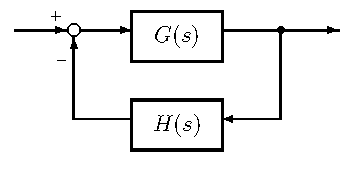
\includegraphics[width=0.5\linewidth]{fig/example.pdf}
  \caption{Example of a figure. }
  \label{fig:fig1}
\end{figure}

\begin{figure}
  \centering
  \begin{subfigure}[b]{0.48\linewidth}
    \centering
    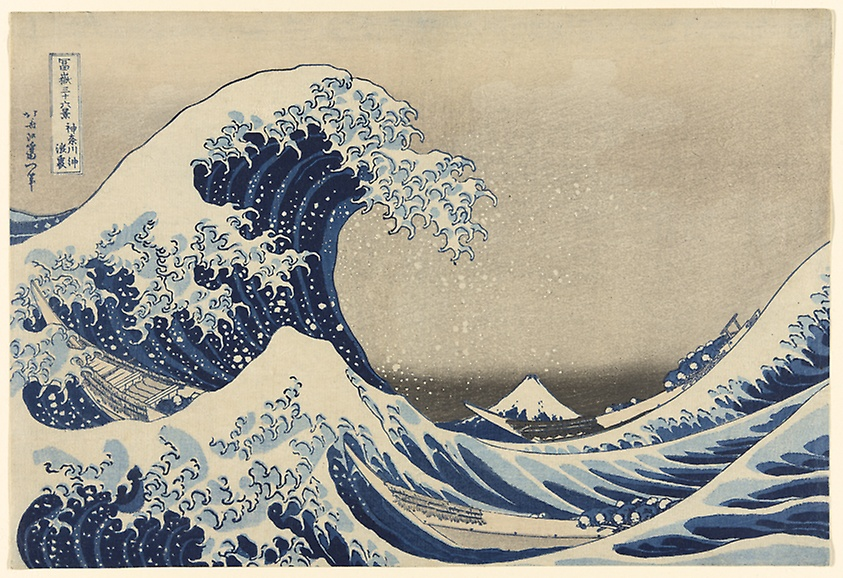
\includegraphics[width=0.98\linewidth]{fig/hokusai.jpg}
    \caption{The Great Wave off Kanagawa. (Raster image.)}
    \label{fig:fig2_a}
  \end{subfigure}
  \begin{subfigure}[b]{0.48\linewidth}
    \centering
    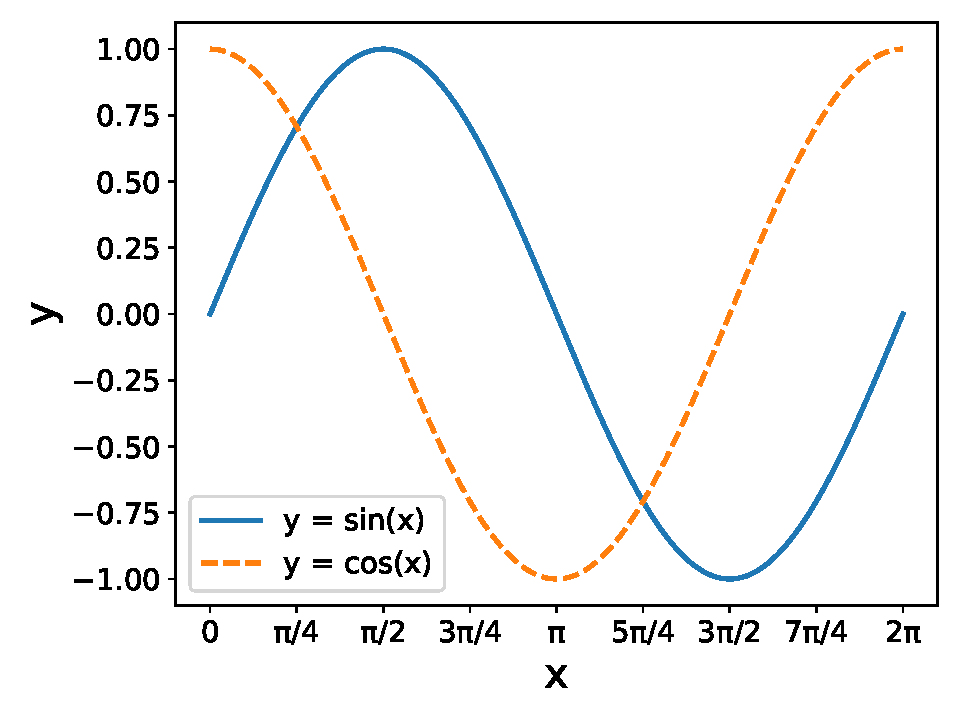
\includegraphics[width=0.98\linewidth]{fig/wave.pdf}
    \caption{Sine and cosine waves. (Vector image.)}
    \label{fig:fig2_b}
  \end{subfigure}
  \caption{Figures of waves. }
  \label{fig:fig2}
\end{figure}

表について,大学のウェブページで配布されている「執筆要綱の補足」では,格子状の罫線が用いられている.
しかし,学術論文では可能な限り表の罫線を省略した方が良いとされ,縦罫線を使用しないことが多い.
縦罫線を使用していない表の例をTable~\ref{tab:table}に示す.
また,\verb|booktabs|パッケージを用いることで,上下の罫線を太くし,適度なスペースを取ってくれる(Table~\ref{tab:booktabs}).
\verb|booktabs|では,罫線の太さや長さなども簡単に変更できる.
一方で,縦罫線の表示を苦手としているので,各々の判断で使用する表のスタイルを選ぶと良い(ただし,論文内で表のスタイルを統一すること).

\begin{table}
  \centering
  \caption{Example of a table. }
  \label{tab:table}
  \begin{tabular}{lrr}
    \hline
    Item   & Price (yen) & Number \\
    \hline
    Apple  & 125         & 5      \\
    Orange & 90          & 10     \\
    Grape  & 320         & 3      \\
    \hline
  \end{tabular}
\end{table}

\begin{table}
  \centering
  \caption{Example of a table using booktabs. }
  \label{tab:booktabs}
  \begin{tabular}{lrr}
    \toprule
    Item   & Price (yen) & Number \\
    \midrule
    Apple  & 125         & 5      \\
    Orange & 90          & 10     \\
    Grape  & 320         & 3      \\
    \bottomrule
  \end{tabular}
\end{table}

図表の配置位置について,\verb|bxjsarticle|の既定値では,\verb|\begin{figure}[tbp]|(ページの上,下,別ページの優先順位)が用いられている.
テキストの間に入れたい場合は,\verb|\begin{figure}[h]|のようにする.


\subsection{数式・単位}

数式の例を式(\ref{eq:equation})に示す.
数式には\verb|amsmath|パッケージを用いる.
\verb|amsmath|パッケージがサポートしていない環境(例えば,\verb|eqnarray|)の使用は避ける.

\begin{equation}
  E=mc^2
  \label{eq:equation}
\end{equation}

また,単位については,執筆要綱にあるように国際単位系(SI)を用いる.
必要に応じて,SI単位を扱うためのパッケージである\verb|siunitx|を用いると良い.


\subsection{脚注}

脚注\footnote{脚注の例をここに示す.}は,\verb|\footnote|によって挿入できる.
執筆要綱には特に記載がないが,参考文献に含めるほどではない情報(例えば,ウェブサイトなど)や付録とするほどでもない補足説明などに用いると良い.


\subsection{参考文献}
\label{sec:reference}

執筆要綱によると,引用文献には通し番号をつける必要がある.
\ref{sec:bst_file}で説明する{\BibTeX}スタイルファイルを用いた場合,引用された順番に参考文献が自動で並び替えられる.
\BibTeX を利用しない場合は,手動で参考文献の記述・並び替えを行うこと.

本文中の引用箇所には,その文献番号を「文献引用箇所$^{(1),\,(2)\,\cdots}$」あるいは「文献引用箇所$^{(1)~(3)}$」のように書く.
\verb|\cite{bib1}|のように記述すると「文献$^{(1)}$」と出力される.
また,\verb|\cite{bib1,bib2,bib3}|のように,複数の文献をまとめて引用した場合,「文献$^{(1),\,(2),\,(3)}$」と出力される.

一般的に,文末に脚注を挿入する場合は句点の後(例えば「…である.$^{*99}$」),参考文献の場合は句点の前(例えば「…である[99].」)に挿入する.
しかし,参考文献の番号を右肩に書く場合,一部の学術雑誌\footnote{
  米国医師会(American Medical Association)や米国化学会(American Chemical Society)の学術雑誌など.
}のように,句点の後に入れると良いだろう(例えば「…である.$^{(99)}$」のように書く).

また,執筆要綱によると参考文献は下記のように書く.
\begin{description}
  \item[学術雑誌等の場合] 著者名,題目,雑誌名,巻数-号数,(西暦で発行年),ペ-ジの順.
  \item[書籍の場合] 著者名,書籍名,(西暦で発行年),ペ-ジ,出版社名の順.
\end{description}


\subsubsection{{\BibTeX}スタイルファイル}
\label{sec:bst_file}

本テンプレートでは,{\BibTeX}スタイルファイルである\verb|kit_mech_thesis.bst|を同梱しており,執筆要綱に準ずる参考文献リストを作成できる.
以下に参考文献の種類ごとの例を示す.

\begin{itemize}
  \item 学術雑誌等の論文(Journal Article, \verb|@article|)の場合\cite{article:en}
  \item 書籍(Book, \verb|@book|)の場合\cite{book:en}
  \item 学会で発表された論文(in Proceedings, \verb|@inproceedings|)の場合\cite{inproceedings}
  \item 書籍の章やセクションなど,書籍の一部(in Collection, \verb|@incollection|)の場合\cite{incollection}
  \item 博士論文(Ph.D. Thesis, \verb|@phdthesis|)の場合\cite{thesis:en,thesis:jp}
  \item 大学,研究機関などから出版された報告書(Technical Report, \verb|@techreport|)の場合\cite{techreport}

  \item 日本語の学術雑誌等の論文(\verb|@article|)の場合\cite{article:jp}
  \item 日本語の書籍(\verb|@book|)の場合\cite{book:jp}

  \item その他(Miscellaneous, \verb|@misc|),例えばインターネット上のウェブサイトの場合\cite{web}
\end{itemize}

\noindent
学術雑誌等(\verb|@article|)および書籍(\verb|@book|)以外は執筆要綱に指示がないので,使用時は注意されたい.
参考文献が適切に出力されているか確認すること.

執筆要項に準ずるのであれば,著者が多い場合「R. E. Edwards, et al.」のように出力すべきである.
BIBファイルの\verb|author|の値を\verb|{Author, First and others}|とすることで,「F. Author, et al.」と出力される.

\subsection{テンプレートの英語化(English Version)}

英語で卒論・修論を書く場合,BXJSクラスの英語化オプションを用いる.
例えば,次のように\verb|\documentclass|に\verb|english|を追加する.

\verb|\documentclass[pdflatex,|{\color{magenta}\verb|english|}\verb|]{kit_mech_thesis}|


\subsection{本テンプレートの上級者向け説明}

本節では,卒論・修論を書くときに知らなくても良いが,テンプレートの調整などに必要となる情報について述べる.


\subsubsection{クラスファイル内で読み込んでいるパッケージについて}
\label{sec:packages}

本テンプレートのクラスファイル(\verb|kit_mech_thesis.cls|)では,BXJSクラスの\verb|bxjsarticle|を\verb|[ja=standard,a4paper,base=11pt,jbase=11pt,nomag*]|のオプションを使用して読み込んでいる.
加えて,下記のパッケージを読み込んでいる.
重複して読み込む場合は注意されたい.

\begin{description}
  \item[\texttt{graphicx}]
        画像を取り込むためのパッケージ.
        {\pLaTeX}/{\upLaTeX}使用時は,\verb|dvipdfmx,hiresbb|のオプションを使用している.
        {\pLaTeX}/{\upLaTeX}以外では,オプションなし.
        (詳しくは,\ref{sec:image_file}を参照されたい.)
  \item[\texttt{hyperref}]
        \verb|\ref|や\verb|\cite|などを用いたとき,PDFファイルにハイパーリンクを作成するためのパッケージ.
        印刷することを考慮して,\verb|hidelinks|オプションを指定しているため,リンクに色や枠が付かない.
  \item[\texttt{tocloft}] 目次をカスタマイズするためのパッケージ.
  \item[\texttt{natbib}] 文献の引用スタイルをカスタマイズするためのパッケージ.
  \item[\texttt{caption}] 図・表のキャプションをカスタマイズするためのパッケージ.
  \item[\texttt{subcaption}] 図を複数並べるためのパッケージ.\verb|caption|パッケージとの互換性がある.
  \item[\texttt{titlesec}] 章・節・項の番号と見出しを太字ゴシック体に変更するために使用.
  \item[\texttt{placeins}] \verb|\section|内の図・表が\verb|\section|よりも前に挿入されるのを防ぐために使用.
  \item[\texttt{footmisc}] 脚注の位置を調整するためのパッケージ.
  \item[\texttt{ifthen}] IF THEN ELSE文やDO WHILE文を使用できるようにするパッケージ.中表紙での卒論・修論の判別に使用.
  \item[\texttt{contour}] 文字に輪郭線を追加できるバッケージ.BXJSクラスではJSクラスと同様に,和文で\verb|\textbf|を用いたとき,ゴシック体に変換される.太字明朝体の代替手法として使用.
  \item[\texttt{plautopatch}]{\pLaTeX}/{\upLaTeX}間のパッケージの競合を防ぐパッケージ({\pLaTeX}/{\upLaTeX}使用時のみ).
\end{description}


\subsubsection{余白の設定について}

BXJSクラスでは,内部で\verb|geometry|パッケージを読み込んでページレイアウトを設定している.
本テンプレートのクラスファイル内では\verb|\setpagelayout|によって,\verb|geometry|の設定の一部を修正し,執筆要綱に基づいたレイアウトにしている.

JSクラスでは,「版面を拡大縮小する」という処理を行っている.
BXJSクラスでも同様な処理を行えるように,\verb|magstyle|オプションが提供されている.
しかし,この処理は{\LuaLaTeX}で使用できない.
コンパイラ間でのPDF出力の差を小さくするため,\verb|magstyle=nomag*|を用いている.

\subsubsection{フォントサイズについて}

「執筆要綱の補足」に従うのであれば,本文のフォントサイズは11~ptとする必要がある.
BXJSクラスでは,JSクラス(\verb|jsarticle|)と同様に \verb|##pt|のオプションでフォントサイズを指定した場合,名前と実際に設定される値がずれているものが多い.
例えば,\verb|11pt|では10.95~ptが実際の設定値となる.
\verb|base=11pt|とすることにより,基底フォントサイズを文字通り11~ptに設定できる.

また,BXJSクラスはJSクラスと同様に,和文フォントが欧文フォントよりもやや小さくなるように設定されている(0.924715倍).
\verb|jbase=11pt|または\verb|scale=1.0|をオプションに追加することにより,和文の基底フォントサイズを11~ptに設定できる.


\subsubsection{図のファイル形式について}
\label{sec:image_file}

{\LaTeX}の画像ファイルでは,EPSファイル(PostScript形式の画像ファイル)がよく用いられている.
通常,{\LaTeX}(または{\pLaTeX},{\upLaTeX})では,TeXファイルからDVIファイルを生成する.
その後,\verb|dvipdfmx|によってDVIからPDFへの変換を行う.
EPSファイルは,\verb|dvips|によってDVIからPostScriptを出力していたころの名残である.
また,{\pdfLaTeX}など,TeXファイルから直接PDFファイルを生成する場合,画像ファイルをEPSからPDFに変換してから最終出力PDFファイルに埋め込む.
したがって,最終出力がPDFファイルであれば,EPSファイルを使うよりも,PDF,PNG,JPEGファイルなどのPDFに直接埋め込めるファイル形式の方が望ましい.

{\pLaTeX}や{\upLaTeX}など,DVIを経由する場合,図形の大きさを示すバウンディングボックス(Bounding Box)の情報が必要になる.
EPSファイルは,バウンディングボックスの情報を持っている.
しかし,PDF,PNG,JPEGなどの画像ファイルは,バウンディングボックス情報を持っていない.
このため,これらのファイルを扱うには,何らかの方法でバウンディングボックス情報を取得し,設定する必要がある.
\verb|graphicx|の\verb|hiresbb|オプションは,画像のバウンディングボックスを高精度で取得するオプションである.
このオプションにより,PDF,PNG,JPEGもEPSファイルと同様な方法で\verb|\includegraphics|によって取り込める.
なお,{\pdfLaTeX}などのDVIを経由せずに直接PDFファイルを生成する方法では,\verb|hiresbb|オプションを設定する必要がない.


\subsubsection{{\BibTeX}スタイルファイルについて}
\label{sec:bib_style}

執筆要綱に記載されている参考文献の書き方は,かなり特殊なものとなっている.
例えば,著者が日本人の場合は氏名フルネームに対して外国人はファースト・ミドルネームがイニシャル,
巻と号の間の区切りがハイフン(--),コンマ区切りが多いなど,基本的な{\BibTeX}スタイルと異なる.
このため,既存の{\BibTeX}スタイルを用いることができず,\verb|kit_mech_thesis.bst|を同梱している.

\verb|kit_mech_thesis.bst|は,\verb|makebst|によって大枠を作成したあと,著者や区切りの処理を修正している.
\verb|makebst|は日本語文献の処理に対応していないため,\verb|junsrt.bst|などを参考に著者情報が漢字かどうかの判別を行う仕組みを実装している.
\verb|kit_mech_thesis.bst|は,力技で実装した部分も多いので,参考文献が適切に出力されているか適宜確認すること.

なお,\verb|biblatex|の方が参考文献のスタイルの修正が容易であるが,日本語環境に対応していない(漢字かどうかの判別フラグを実装できない)ため,今回は使用していない.


\subsection{{\pdfLaTeX}と{\XeLaTeX}の日本語の処理について}
\label{sec:latex_comp}

本テンプレートでも使用しているBXJSクラスを{\pdfLaTeX}によってコンパイルするとき,日本語の処理にCJKパッケージである\verb|bxcjkjatype|を用いている.
このCJKパッケージには自動で和欧文間空白を入れる機能がないことに留意されたい(Fig.~\ref{fig:pdflatex}).

{\XeLaTeX}は,日本語の処理がやや苦手のようで,Fig.~\ref{fig:xelatex}のように小書き文字の直前に改行が入りやすい.

\begin{figure}[b]
  \centering
  \begin{subfigure}[b]{0.48\linewidth}
    \centering
    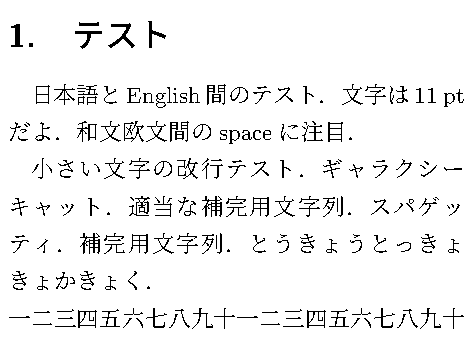
\includegraphics[width=0.98\linewidth]{fig/latex_comp/uplatex.pdf}
    \caption{{\upLaTeX}.}
    \label{fig:uplatex}
  \end{subfigure}
  \hfill
  \begin{subfigure}[b]{0.48\linewidth}
    \centering
    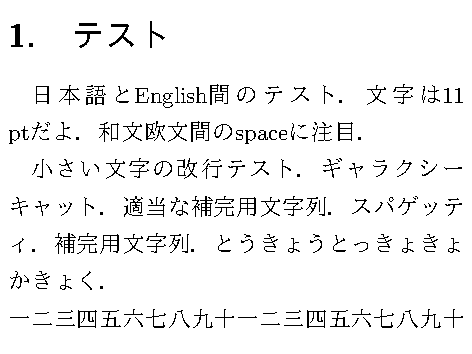
\includegraphics[width=0.98\linewidth]{fig/latex_comp/pdflatex.pdf}
    \caption{{\pdfLaTeX}.}
    \label{fig:pdflatex}
  \end{subfigure}
  \\
  \begin{subfigure}[b]{0.48\linewidth}
    \centering
    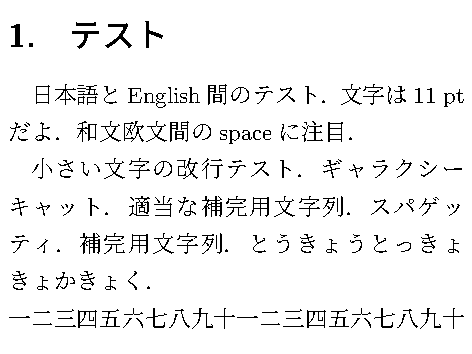
\includegraphics[width=0.98\linewidth]{fig/latex_comp/lualatex.pdf}
    \caption{{\LuaLaTeX}.}
    \label{fig:lualatex}
  \end{subfigure}
  \hfill
  \begin{subfigure}[b]{0.48\linewidth}
    \centering
    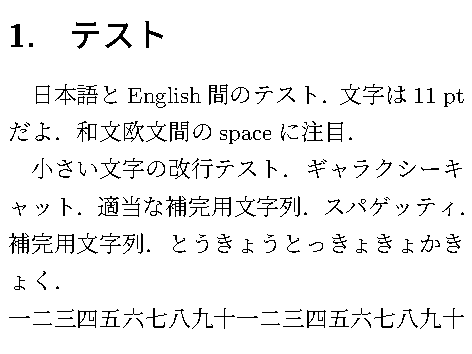
\includegraphics[width=0.98\linewidth]{fig/latex_comp/xelatex.pdf}
    \caption{{\XeLaTeX}.}
    \label{fig:xelatex}
  \end{subfigure}
  \caption{Comparison of PDF output from BXjscls using different {\LaTeX} processing systems.}
  \label{fig:latex_comp}
\end{figure}



% 改ページ
\clearpage
% \input{src/sec_1.tex}
% \input{src/sec_2.tex}


%%%%% 謝辞 %%%%%
\section*{謝辞}
\addcontentsline{toc}{section}{謝辞}  % 謝辞を目次に追加

謝辞には次のような内容を入れると良い.
まず,指導教員(主任指導教員)への感謝を述べる.
副指導教員など,論文執筆にあたりお世話になった教員への感謝を述べる.
共同研究機関や研究で使った施設(オープンファシリティセンターものづくりユニットなど)など,お世話になった機関・施設やその職員がいるのであれば感謝を述べる.
研究室の仲間への感謝を述べる.
論文の研究を行うための研究助成を受けたのであれば,それについても述べる.
家族など支えてくれた方への感謝を述べる.


% 改ページ
\clearpage
\clearpage

%%%%% 参考文献 %%%%%
\addcontentsline{toc}{section}{\bibname} % 参考文献を目次に追加

%% BibTeX 使用者 %%
\bibliographystyle{kit_mech_thesis}
\bibliography{example.bib} % ご自身のbibファイル名を入れる

%% 手入力愛好者 %%
% \begin{thebibliography}{10}
%     \bibitem{bib1}
%     日本太郎, 赤坂次郎, 粘弾性流のレオロジ方程式に関する研究, 
%     日本機械学会論文集, 70--578, (1967), 359--363.
%     \bibitem{bib2}
%     R. E. Edwards, et al., Waterhammer Analysis of Pump System, 
%     Trans. ASME, Ser.E., 30--3, (1969), 384--390.
%     \bibitem{bib3}
%     青山四郎, 自動制御理論, 
%     (1968), 294-300, 機学社.
%     \bibitem{bib4}
%     W. R. Ahrendt and J. F. Taplin, Automatic Feedback Control, 
%     (1968), 31-40, McGraw-Hill, N.Y.
% \end{thebibliography}

\clearpage

\backmatter % 章と図表の通し番号をリセット(主に付録のための処理)

%%%%% 付録 %%%%%
\appendix
\renewcommand{\thefigure}{\Alph{section}\arabic{figure}} % 図の番号を A1, A2, A3, ... に変更
\renewcommand{\thetable}{\Alph{section}\arabic{table}} % 表の番号を A1, A2, A3, ... に変更
% \renewcommand{\thefigure}{\Alph{figure}} % 図の番号を A, B, C, ... に変更
% \renewcommand{\thetable}{\Alph{table}} % 表の番号を A, B, C, ... に変更
\section{付録のタイトル}
\label{sec:appendix_a}
% \addcontentsline{toc}{section}{\appendixname} % 付録が目次に表示されない場合に使用

これは付録の例である.
付録の表記は「付録A,付録B,付録C,...」のように表示され,図表の番号は「A1, A2, A3, ...」(付録のアルファベット+付録内の通し番号)と表示される.

付録が一つのみである場合,「付録A,付録B,付録C,...」のように分ける必要はない.
この場合,\verb|\section|を\verb|\section*|に書き換えると良い.
付録が目次に表示されなくなった場合,\verb|\addcontentsline{toc}{section}{\appendixname}|を用いる.
図表の番号は,\verb|\renewcommand{\thefigure}{\Alph{figure}}|のようにすると,「Fig.~A, Fig.~B, Fig.~C, ...」と表示される.

\begin{figure}
  \centering
  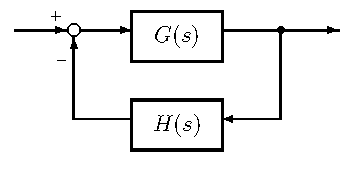
\includegraphics[width=0.6\textwidth]{fig/example.pdf}
  \caption{Figure in the appendix.
    This is an example of a very long caption.
    \lipsum[1]}
  \label{fig:appendix}
\end{figure}

\begin{table}
  \centering
  \caption{Table in the appendix.}
  \label{tab:appendix}
  \begin{tabular}{lrr}
    \hline
    Item   & Price (yen) & Number \\
    \hline
    Apple  & 125         & 5      \\
    Orange & 90          & 10     \\
    Grape  & 320         & 3      \\
    \hline
  \end{tabular}
\end{table}

% 改ページ
\clearpage



\end{document}
